\section{Implementation} \label{s:impl}
We implement the time-indexed based general ILP in \S\ref{s:ilp} and a greedy list scheduling algorithm in \S\ref{s:lst}. The program takes the specification of job weights vector, processing time vector, precedence constraints 0-1 matrix (each $(i, j)$ with entry value 1 indicates $i$ precedes $j$) and number of machines as input, and outputs the weighted sum of completion time, obtained by both ILP and greedy list scheduling. The program can be used for benchmarking approximation algorithms for $P|prec|\sum w_j C_j$ in practice. The code is also open-sourced in \url{https://github.com/hongzimao/6.854/tree/master/project/code}.

We use the implementation to conduct a small scale experiment mainly for the results in \cite{schulz2011near} on the 0-1 bipartite instance. We first did a speed test on ILP approach and the greedy list approach, with a 3 parallel machine scenario, where precedence constraints on a direct acyclic graph is randomly generated with number of constraints is uniformly distributed in $[n/2, n]$ where $n$ is the number of jobs. The weights and processing time are uniformly distributed in $[1, 10]$. We then extend to run 100 experiments each on case with number of jobs $n = [10, 15, 20, 25, 30]$. Figure \ref{fig:obj_ratio} shows the run time comparison averaged over the 100 experiments. As expected, we already see the trend of exponential growing run time in ILP compared with a relatively constant $O(n)$ run time of the list scheduling algorithm.

\begin{figure}[h]
	\centering
	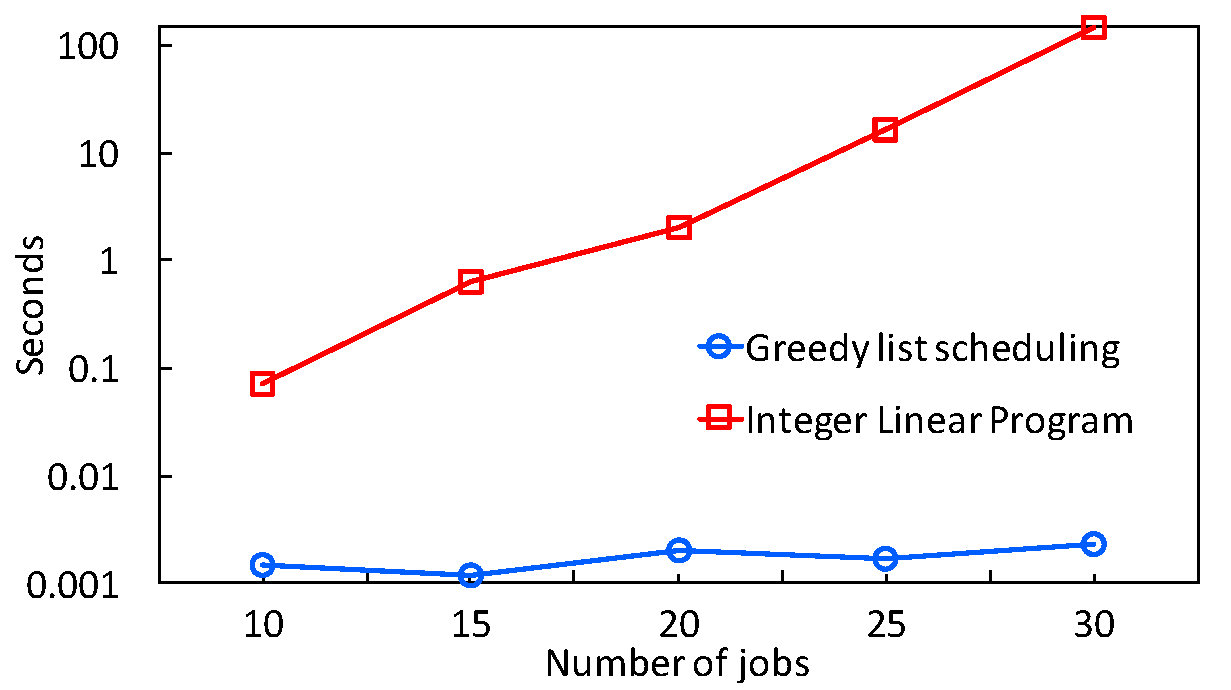
\includegraphics[width=0.6\textwidth]{figs/runtime.pdf}
	\caption{Running time comparison of ILP and simple greedy list scheduling.}
	\label{fig:runtime}
\end{figure}

Then we compare the objective ratio between the list scheduling approximation algorithm and ILP. In a general case of $P|prec|\sum w_j C_j$, as we see in the examples in \S\ref{s:lst} and \S\ref{s:lpc}, that we would expect to see the objective ratio between a quickly computed feasible solution and ILP to increase as the number of job grows. In contrast, \S\ref{s:bism} shows the optimality of random solutions as the number of job increases. In our experiment, we accordingly fix a single machine scenario. Then in 100 experiments for different number of jobs, we randomly assign half of the job to $N_1$ and the other half to $N_2$. For each bipartite pair in $N_1$ and $N_2$, a precedence constrain is established with $0.5$ probability (This satisfies how \S\ref{s:bism} constructs the balanced class.). Then we compare the result with the one in experiment of 3 machine general case in figure \ref{fig:obj_ratio}. The experiment matches with what we expect for the approximation bounds.

\begin{figure}[h]
	\centering
	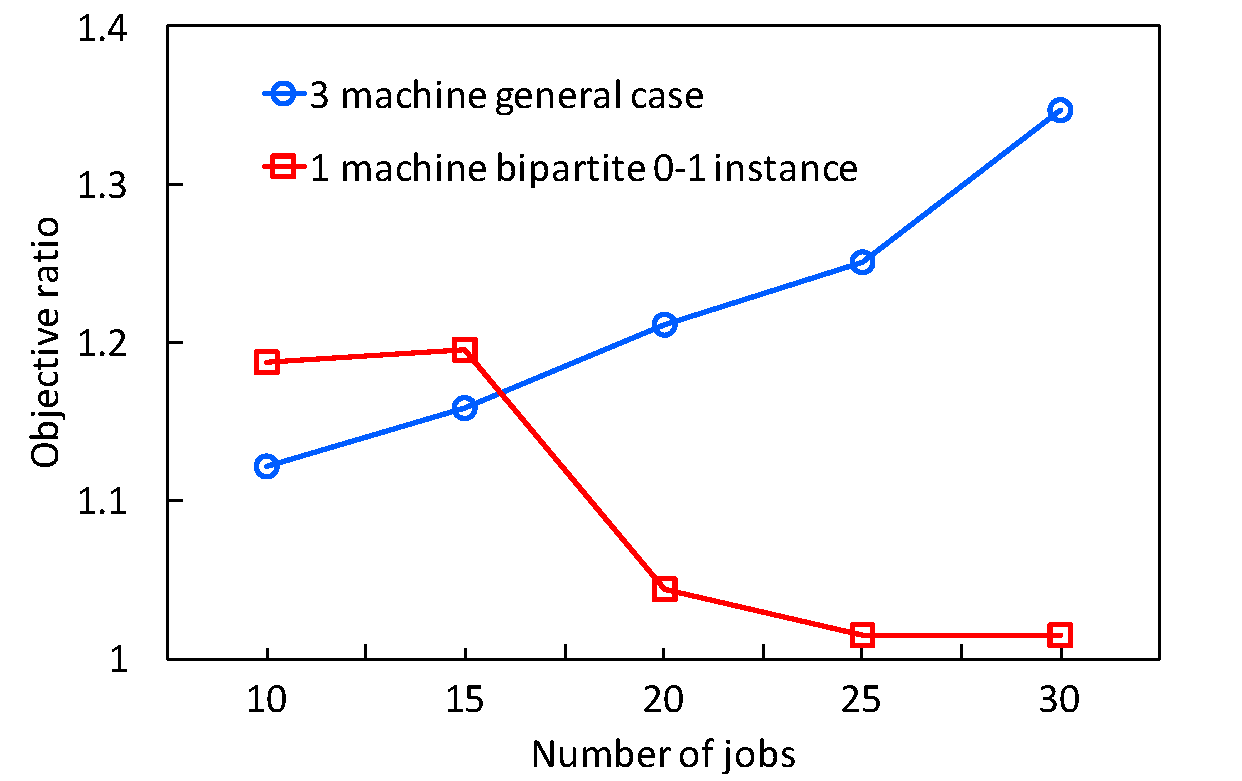
\includegraphics[width=0.6\textwidth]{figs/obj_ratio.pdf}
	\caption{Objective ratio of greedy list scheduling over ILP, on the general 3 parallel machine case and the special bipartite 0-1 instance.}
	\label{fig:obj_ratio}
\end{figure}
